\documentclass[draft]{article}
\usepackage{lmodern}
\usepackage{amssymb,amsmath}
\usepackage{ifxetex,ifluatex}
\usepackage{fixltx2e} % provides \textsubscript
\ifnum 0\ifxetex 1\fi\ifluatex 1\fi=0 % if pdftex
  \usepackage[T1]{fontenc}
  \usepackage[utf8]{inputenc}
\else % if luatex or xelatex
  \ifxetex
    \usepackage{mathspec}
  \else
    \usepackage{fontspec}
  \fi
  \defaultfontfeatures{Ligatures=TeX,Scale=MatchLowercase}
\fi
% use upquote if available, for straight quotes in verbatim environments
\IfFileExists{upquote.sty}{\usepackage{upquote}}{}
% use microtype if available
\IfFileExists{microtype.sty}{%
\usepackage{microtype}
\UseMicrotypeSet[protrusion]{basicmath} % disable protrusion for tt fonts
}{}
\usepackage[margin=1in]{geometry}
\usepackage{hyperref}
\hypersetup{unicode=true,
            pdftitle={The value of information for woodland management: updating a state and transition model},
            pdfauthor={William K. Morris\^{}\{\textbackslash{}dagger,1\}, Michael C. Runge\^{}2 \& Peter A. Vesk\^{}1},
            pdfborder={0 0 0},
            breaklinks=true}
\urlstyle{same}  % don't use monospace font for urls
\usepackage{natbib}
\bibliographystyle{ea.bst}
\usepackage{longtable,booktabs}
\usepackage{graphicx,grffile}
\makeatletter
\def\maxwidth{\ifdim\Gin@nat@width>\linewidth\linewidth\else\Gin@nat@width\fi}
\def\maxheight{\ifdim\Gin@nat@height>\textheight\textheight\else\Gin@nat@height\fi}
\makeatother
% Scale images if necessary, so that they will not overflow the page
% margins by default, and it is still possible to overwrite the defaults
% using explicit options in \includegraphics[width, height, ...]{}
\setkeys{Gin}{width=\maxwidth,height=\maxheight,keepaspectratio}
\IfFileExists{parskip.sty}{%
\usepackage{parskip}
}{% else
\setlength{\parindent}{0pt}
\setlength{\parskip}{6pt plus 2pt minus 1pt}
}
\setlength{\emergencystretch}{3em}  % prevent overfull lines
\providecommand{\tightlist}{%
  \setlength{\itemsep}{0pt}\setlength{\parskip}{0pt}}
\setcounter{secnumdepth}{5}

%%% Use protect on footnotes to avoid problems with footnotes in titles
\let\rmarkdownfootnote\footnote%
\def\footnote{\protect\rmarkdownfootnote}

%%% Change title format to be more compact
\usepackage{titling}

% Create subtitle command for use in maketitle
\newcommand{\subtitle}[1]{
  \posttitle{
    \begin{center}\large#1\end{center}
    }
}

\setlength{\droptitle}{-2em}
  \title{The value of information for woodland management: updating a state and
transition model}
  \pretitle{\vspace{\droptitle}\centering\huge}
  \posttitle{\par}
  \author{William K. Morris\(^{\dagger,1}\), Michael C. Runge\(^2\) \& Peter A.
Vesk\(^1\)}
  \preauthor{\centering\large\emph}
  \postauthor{\par}
  \date{}
  \predate{}\postdate{}

\usepackage{titlesec}
\setcitestyle{aysep={}}
\titleformat{\paragraph}{\small\normalfont\bfseries}{}{0pt}{}
\titleformat{\subparagraph}{\small\normalfont}{}{0pt}{}
\linespread{2}\selectfont
\usepackage{booktabs}
\usepackage{setspace}
\usepackage{caption}
\usepackage{tikz}
\usepackage{pdflscape}
\captionsetup{font={stretch=2}}
\usepackage{pbox}
\usepackage[nomarkers]{endfloat}
\renewcommand{\listoffigures}{}
\renewcommand\bibname{Literature Cited}

\usepackage{amsthm}
\newtheorem{theorem}{Theorem}[section]
\newtheorem{lemma}{Lemma}[section]
\theoremstyle{definition}
\newtheorem{definition}{Definition}[section]
\newtheorem{corollary}{Corollary}[section]
\newtheorem{proposition}{Proposition}[section]
\theoremstyle{definition}
\newtheorem{example}{Example}[section]
\theoremstyle{definition}
\newtheorem{exercise}{Exercise}[section]
\theoremstyle{remark}
\newtheorem*{remark}{Remark}
\newtheorem*{solution}{Solution}
\begin{document}
\maketitle

$\dagger$ Corresponding author: wkmor1@gmail.com\\
1. School of BioSciences, the University of Melbourne, Parkville 3010, Victoria.\\
2. Patuxent Wildlife Research Center, US Geological Survey, Laurel, MD 20708.

\newpage

\section*{Abstract}\label{abstract}
\addcontentsline{toc}{section}{Abstract}

Value of information (VOI) analyses reveal the expected benefit of reducing uncertainty to a decision maker. Most ecological VOI analyses have focused on population models rarely addressing more complex community models. We performed a VOI analyses for a complex state and transition model of Box-Ironbark Forest and Woodland management. With three management alternatives (limited harvest/firewood removal, ecological thinning and no management), managing the system optimally (for 150 years) with the original information, would on average, increase the amount of forest in a desirable state from 19 to 35\% (a 16 percentage point increase). Resolving all uncertainty would, on average, increase the final percentage to 42\% (a 19 percentage point increase). However, only resolving the uncertainty for a single parameter was worth almost two-thirds the value of resolving all uncertainty. We found the VOI to depend on the number of management options, increasing as the management flexibility increased. Our analyses show it is more cost-effective to monitor low-density regrowth forest than other states, and more cost-effective to experiment with the no management alternative than the other management alternatives. Importantly, the most cost-effective strategies did not include either the most desired forest states, nor the least understood management strategy, ecological thinning. This implies that managers cannot just rely on intuition to tell them where the most value of information will lie, as critical uncertainties in a complex system are sometimes cryptic.

Keywords: Box-Ironbark, decision theory, monitoring, multivariate adaptive regression splines, optimization.

\section*{Introduction}\label{introduction}
\addcontentsline{toc}{section}{Introduction}

Ecosystems are typically managed under uncertainty. Reducing uncertainty
(through monitoring, experiments, or other research) can facilitate
management decisions with greater expected benefits. On the other hand,
sometimes reducing uncertainty is not justified
\citep{Mcdonaldmadden2010}. The decision to gather new information is
only rational if the expected benefit when making a decision with new
information outweighs the cost of learning. Determining the value of
information facilitates calculating this benefit \citep{Raiffa1961}.

Value of information (VOI) theory is a set of decision theoretic tools
that have previously been applied to decision problems in economics,
medicine, engineering and other domains
\citep{Dakins1999, Yokota2004a, Claxton2008, Wu2013, Keisler2014}. With
the VOI toolset, a decision analyst can assess what to monitor, how much
to monitor and even whether monitoring is justified at all.

Compared with other fields, such as operations research and medicine,
ecology and natural resource management have been slower to adopt VOI
analyses for decision making, although recently, some examples have
appeared in the literature
\citep[e.g.,][]{Polasky2001, Moore2011, Runge2011a, Runting2013}. Most
examples have focused on evaluating VOI for models with discrete
expressions of model uncertainty \citep[e.g.,][]{Moore2012}.
Furthermore, ecological decision problem solvers have tended to focus on
models of population dynamics
\citep{Runge2011a, Johnson2014a, Canessa2015, Maxwell2015} rather than
community and/or ecosystem-level models. This is an important gap in our
understanding, as much effort and resources are expended on ecosystem
management. \citet{Kangas2010} noted the potential for VOI to help
foresters target data acquisition. More recently, \citet{Roessiger2016}
have shown that using more optimally informed models of forest stand
dynamics improves the outcomes of management.

One reason why communities and ecosystems have rarely been the focus of
VOI analyses is that community or ecosystem models make VOI analysis
difficult to perform. Ecosystem models, such as state and transition
models (STM), exhibit complex nonlinear dynamics, have many parameters
(multidimensional), and their uncertainties are often continuous, rather
than discrete, making it difficult to calculate the VOI analytically. By
continuous and discrete uncertainty, we mean to distinguish between
continuous uncertainty that takes on infinite values (such as the
uncertainty described by a normal density function) and discrete
uncertainty that ascribes probabilities to some finite set of values.

An approach to dealing with multidimensional continuous uncertainty and
avoid having to contend with the complex integral calculus needed to
perform a VOI analytically, is to simplify the problem by representing
the uncertainty with a set of discrete values. Here we introduce a case
study on VOI for a complex, high-dimensional model with underlying
continuous uncertainty represented by sets of discrete parameter values.
For the present analysis we purposely avoid the issue of non-linear
temporal dynamics and only set out to address the problems of
high-dimensionality and continuous uncertainty, leaving this third
potential source of complexity for another forum.

In the work that follows we briefly introduce our motivating example of
Box Ironbark Forest and Woodland (BIFAW) management and revisit the
state transition models of this system built by \citet{Czembor2009}. We
then provide the reader with some introductory material on VOI analyses
and its variants, before applying these techniques to our case study and
demonstrate how some of the inherent complexities can be addressed by
discretising the uncertainty and applying stepwise algorithms that
negate the need for complex integral calculus. The overarching aim of
this work is to demonstrate how to apply and interpret a VOI analysis
for a complex ecosystem model with many parameters. While the methods we
use could be applied to a broad range of ecological decision problems,
the results we see are sensitive to the specific objectives, model and
initial state of uncertainty we confront below.

\subsection*{Box Ironbark Forest and Woodland
management}\label{box-ironbark-forest-and-woodland-management}
\addcontentsline{toc}{subsection}{Box Ironbark Forest and Woodland
management}

The BIFAW region covers approximately 250,000 ha of central Victoria,
Australia. The BIFAW are plant communities that occur on low-fertility
soils and in a semi-arid to temperate climate. Much of the pre-19th
century stands of BIFAW were cleared for agriculture and gold mining.
Most of the current extent is highly fragmented regrowth. These regrowth
stands are typically missing key ecosystem components such as large,
hollow-bearing trees and a diverse understory shrub layer. Tree species
found in BIFAW include Grey Box (\emph{Eucalyptus microcarpa}), Red Box
(\emph{E. polyanthemos}), Long Leaf Box (\emph{E. goniocalyx}), Yellow
Box (\emph{E. melliodora}), Red Ironbark (\emph{E. tricarpa}), Red
Stringybark (\emph{E. macrorhyncha}) and Yellow Gum (\emph{E.
leucoxylon}). The BIFAW supports important habitat for three
Victorian-listed threatened taxa: Brush-tailed Phascogale
(\emph{Phascogale tapoatafa}), Powerful Owl (\emph{Ninox strenua}) and
Regent Honeyeater (\emph{Xanthomyza phrygia}) \citep{Tzaros2005}. The
latter is also a federally listed endangered species. Regent Honeyeaters
are threatened because they rely on large trees for foraging and nesting
\citep{Menkhorst1999}.

In 1996 the state government of Victoria commissioned an investigation
into an appropriate system for the protection and management of BIFAW.
As a direct result, over 200,000 ha of BIFAW were gazetted as national
park and other protected areas. The report recommended a program of
ecological thinning be undertaken as part of an ecological management
strategy to assist the development of a forest structure ultimately
dominated by large diameter trees in the new parks and reserves
\citep{ECC2001, Pigott2009}. Ecological thinning is the active reduction
of stem density by removing select trees from the stand. Stands are
thinned to a density that approximates the density of an older stand.
The reduction in density aims to improve forest health as the remaining
trees have greater resource availability and faster growth rates are
presumed. In addition, some of the fallen timber resulting from the
thinning is retained to improve habitat for plants and animals
\citep{Cunningham2009, Horner2010}. In 2003 the body in charge of BIFAW
park management, Parks Victoria, established an ecological thinning
trial. The aim of the trial was to investigate whether ecological
thinning could be used to restore structural diversity of habitat types
and the functioning and persistence of key communities and species
populations \citep{Pigott2010}. Short-term observations imply that a
diverse shrubby understory is enhanced under a program of ecological
thinning \citep{Jones2015}.

\subsubsection*{State and transition models of Box Ironbark Forest and
Woodland}\label{state-and-transition-models-of-box-ironbark-forest-and-woodland}
\addcontentsline{toc}{subsubsection}{State and transition models of Box
Ironbark Forest and Woodland}

\citet{Czembor2009} built a suite of simulation models of BIFAW dynamics
with parameters estimated through expert elicitation using methods
adapted from \citet{Morgan1990}. Their BIFAW state and transition models
predict the proportions of a model landscape in four states:
high-density regrowth (HDRG), low-density regrowth (LDRG), and the two
states most desired by land-managers, mature high-density woodland
(MHDW), and mature low-density woodland (MLDW). The models included
three management options, no management/natural disturbance only (NM),
limited harvest/firewood removal (HF), and ecological thinning (ET).
Briefly, the models predict the state of the landscape through time by
applying a transition matrix that differs according to the management
action applied \citep[see methods,][ for more
information]{Czembor2009, Czembor2011}. The simulation models the
dynamics of 1000 1ha spatially implicit cells.

We make the simplifying assumption that the dynamics of the system are
linear with respect to the actions taken. That is, they lack
interactions that make the outcome of one action depend on the
application of any other action. In effect, there were separate models
for each of the actions, one model that predicted the dynamics (changes
in state through time) of the BIFAW when NM was applied, one model for
HF and one for ET. While a more complex model that included the extra
layer of dynamism and included non-linear relationships between
combinations of actions and outcome may have produced more realistic
results, the simplification was necessary to facilitate the expert
elicitation used to parameterise the models.

\subsubsection*{Uncertainty in Box Ironbark Forest and Woodland
models}\label{uncertainty-in-box-ironbark-forest-and-woodland-models}
\addcontentsline{toc}{subsubsection}{Uncertainty in Box Ironbark Forest
and Woodland models}

Analyzing the variation among models which included three components of
uncertainty, \citet{Czembor2011} found that between-expert uncertainty
was the greatest contributor to total model uncertainty, followed by
imperfect individual expert knowledge, then system stochasticity. In the
case presented here we treated the opinions of the experts as the
initial state of uncertainty---the original information.

Uncertainty in STM parameters can be represented by a continuous
multidimensional (where the dimensions are the different model
parameters) probability distribution. However, the elicitation process
used by Czembor et al, yields an approximation of such a distribution in
the form of multiple discrete estimates of each parameter (in this case,
375 estimates per parameter) that represents the underlying continuous
expression of uncertainty. With the discrete estimates of the parameter
values we can summarise the continuous parameter space, in much the same
way as a histogram of samples represents some underlying probability
distribution.

\subsection*{Decision problem}\label{decision-problem}
\addcontentsline{toc}{subsection}{Decision problem}

The fundamental objective of the BIFAW region managers is to ensure the
persistence of key, functioning communities and species populations of
the region. Managers have determined that the means of achieving these
objectives is to maximize the proportion of the landscape in a mature
woodland (either high, MHDW, or low-density, MLDW) state which supports
key habitat components such as hollow bearing trees and a diverse
shrubby understory. They have three management actions available to
achieve this objective: no management/allow natural disturbance only
(NM), allow limited harvest/firewood removal (HF) and thinning (ET).
Importantly for the models of Czembor et al, the actions are applied
initially and only once, then the models track the state transitions of
the modelled BIFAW units (spatially implicit cells) through time.

The objective is to maximize the proportion of the BIFAW in either
low-density or high-density mature woodland after 150 years, by finding
the optimal management action to apply to each cell initially. More
formally, the objective can be written as:

\begin{equation}
\begin{aligned}
&\textrm{max}_\textrm{NM,HF,ET}(\textrm{MHDW}_{t = 150} + \textrm{MLDW}_{t = 150})\\
\textit{subject to}&\\
&\textrm{ET} < 0.2\\
&\textrm{NM} + \textrm{HF} + \textrm{ET} < 1 
\end{aligned}
\label{eq:obj}
\end{equation}

As the model is spatially implicit it does not account for the spatial
arrangement of management action and so the dynamics are only effected
by the proportion of cells subject to each management action. To
represent the practical limitations on the resources available for
management, we placed a constraint that only 20\% of the BIFAW can be
thinned. However, we also test the effect of applying this constraint by
varying the allowable proportion of thinning from 10 to 100\%.

The case study, as outlined here, falls in class of problems known as
linear optimizations. As such, the solutions to the objective
maximization will always lie on one of the vertices of the feasible
region of management. In other words, the action that maximizes the
objective will be be either 100\% NM, 100\% HF, 20\% ET and 80\% NM or
20\% ET and 80\% HF (or the equivalent proportions when the constraint
on ET is different; \ref{fig:Figure1}). Here it is important to note
that if the additional dynamic complexity of between action interaction
had been modelled (as discussed above) then this assumption of linearity
could not be made and any combination of actions may potentially be
optimal.





\begin{figure}[htbp]
\centering
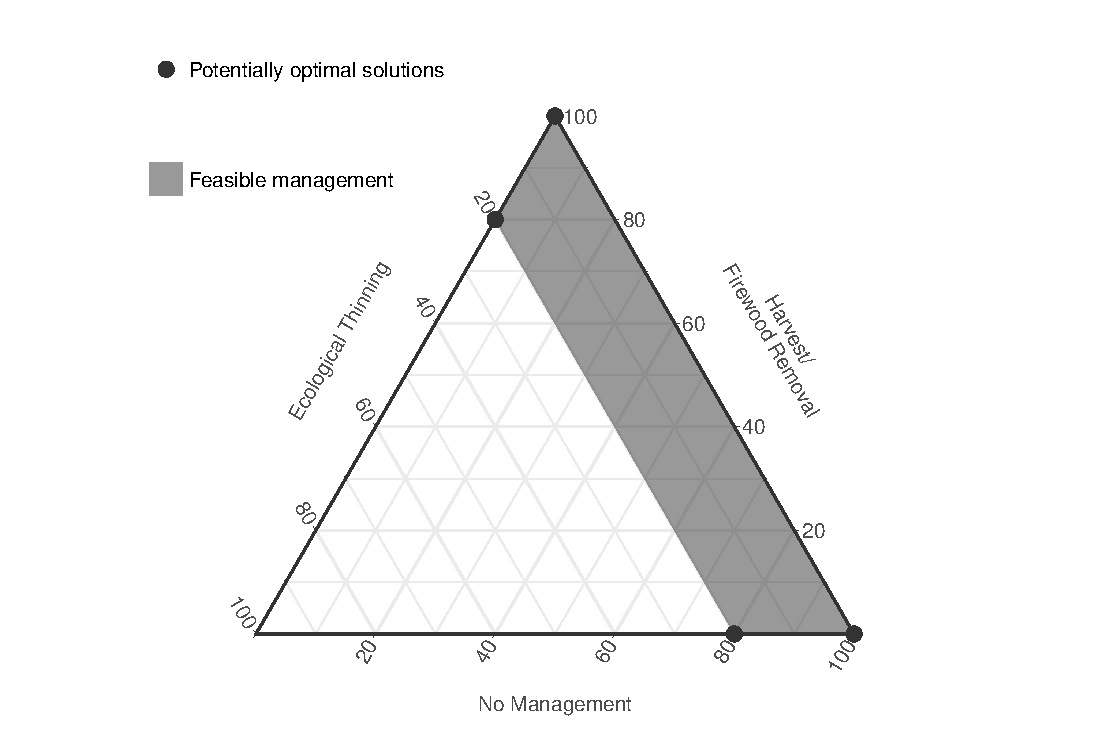
\includegraphics{Figure1-1.pdf}
\caption{\label{fig:Figure1}Ternary diagram highlighting the feasible region of
management (maximum allowed thinning of 20\%) and the four vertices
representing potential optimal solutions to the decision problem.}
\end{figure}

\subsection*{Calculating the value of
information}\label{calculating-the-value-of-information}
\addcontentsline{toc}{subsection}{Calculating the value of information}

A value of information analysis can be used to assess the benefit of
reducing epistemic uncertainty before making a decision. A decision
analyst cannot know, in advance, what information they will gain if they
seek to learn before taking action. The expected value \emph{of}
information (EVI) is the difference between the expected value with
\emph{new} information (EVWNI) and the expected value with
\emph{original} information (EVWOI). The EVI can come in a number forms
depending on the form of new information. Regardless of form, all
variants of EVI analyses assume decisions are being made optimally. That
is, the decision analyst considers value to arise from taking actions
that maximize the expected value given the original or new information.
To do so, the decision analyst requires a model that can be used to
predict the outcomes of possible future decisions. In calculating EVI,
the analyst will use such a model to predict decision outcomes using the
original or new information as their model inputs.

As noted above, value of information can take multiple forms. Here we
deal with two forms: the expected value of perfect information (EVPI)
and the partial expected value of perfect information (EVPXI). Where X
in this case indicates the component of information that will be known
perfectly. Here we will briefly outline the general form of an EVI
analysis in terms of EVPI and EVPXI. For a more detailed description of
the derivation of EVI and its variants, see the seminal text of
\citet{Raiffa1961} and for more recent treatments see
\citet{Yokota2004a} and \citet{Williams2011}.

The expected value of perfect information (EVPI) quantifies the expected
performance gain if all uncertainty is resolved prior to taking action
\citep{Raiffa1961}. The EVPI is the upper bound of expected performance
improvement and can identify the amount of resources worth investing to
resolve uncertainty \citep{Runge2011a}. While EVPI provides a value for
complete reduction of uncertainty, EVPXI can quantify the performance
gain if uncertainty is only partially resolved \citep{Ades2004}.

Again, the EVI is the difference between the EVWNI and the EVWOI. When
the new information is perfect (i.e., the analyst's model will have all
uncertainty eliminated) then it follows that:

\begin{equation}
\mathrm{EVPI} = \mathrm{EVWPI} - \mathrm{EVWOI}
\label{eq:EVWOIch1}
\end{equation}

where EVWPI is the expected value \emph{with} perfect information.

To calculate the expected values EVWPI and EVWOI, like any expected
value, the analyst will work out the value they expect to see on average
when taking the most optimal, or maximizing actions. More formally:

\begin{equation}
\mathrm{EVWOI} = Max_{a}[Mean_{s}(Value)]
\label{eq:EVWOIch1}
\end{equation}

and

\begin{equation}
\mathrm{EVWPI} = Mean_{s}[Max_{a}(Value)]
\label{eq:EVWPIch1}
\end{equation}

Where \(a\) indicates the actions available and \(s\) indicates the
initial uncertainty or the state space (the world of possible scenarios
that could lead an action to generate some value). As you can see, both
the equations for EVWPI and EVWOI are similar. The key difference is the
order of maximization (optimizing) and averaging (taking the mean over
the uncertainty). Calculating the EVPXI requires a similar yet more
complicated approach. For a model with multiple parameters, to calculate
the EVPXI for the \(i^{th}\) parameter(s) of interest is expressed
formally as:

\begin{equation}
\mathrm{EVPXI_i} = \mathrm{EVWPXI_i} - \mathrm{EVWOI}
\label{eq:EVPXIch1}
\end{equation}

where,

\begin{equation}
\mathrm{EVWPXI_i} = Mean_{s_i}\{Max_{a}[Mean_{s_c}(Value)]\}
\label{eq:EVWPXIch1}
\end{equation}

Here \(c\) represents the rest of the parameters in the model with
uncertainty, \(s\). Partial perfect information requires an additional
averaging-over step, where value is averaged over the \(c^{th}\)
not-of-interest parameters, then maximization occurs, before finally
averaging over the initial uncertainty of the parameter(s) of interest
takes place.

\subsection*{Study objectives}\label{study-objectives}
\addcontentsline{toc}{subsection}{Study objectives}

In the following work we apply the above calculations of EVPI and EVPXI
to the BIFAW model to ascertain whether and how the addition of new
information may improve the outcome of their management. To find the
upper bound on the value of information we calculated the expected value
of perfect information (EVPI) for the BIFAW model. We then calculated
the the partial value of perfect information (EVPXI) for all transition
probabilities to determine which parameters have the greatest value for
learning.

We also analysed a set of sampling strategies that resolved the
uncertainty for multiple parameters simultaneously. To do so, we
calculated the EVPXI for two parameters at a time. First we calculated
two-parameter EVPXI for parameters pertaining to specific system states.
Second we did the same for parameters pertaining to each management
action (see methods section for further details). Finally we tested the
effect of varying a constraint on action to see what happened to the
expected value of information when the options available to a manager
changed.

\section*{Methods}\label{methods}
\addcontentsline{toc}{section}{Methods}

\subsection*{Predicting the outcome of management under
uncertainty}\label{predicting-the-outcome-of-management-under-uncertainty}
\addcontentsline{toc}{subsection}{Predicting the outcome of management
under uncertainty}

The system model we used to make predictions of BIFAW management
decision outcomes were multivariate adaptive regression splines (MARS)
fit to the output data from the STMs of \citet{Czembor2011}. MARS is a
non-parametric regression technique extending linear models. A MARS
model is a weighted sum of a set of basis functions which include
constants and hinge functions. As a result MARS models can incorporate
non-linearities and interactions. MARS models are fit with a two-step
algorithm starting with a forward pass in which the basis functions are
iteratively added to the model. In the second step, the backward pass,
the basis functions are pruned using cross-validation thus reducing
overfitting \citep{Friedman1991}. We chose to represent the state and
transitions using MARS rather than run further STMs as the latter would
be computationally infeasible given the large number of repeated model
runs needed for the analyses.

The STMs predicted the proportion of the modelled BIFAW landscape in
four vegetation states after 150 years. Again, the four states in the
models were high-density regrowth (HDRG), low-density regrowth (LDRG),
high-density mature woodland (HDMW), and low-density mature woodland
(MLDW). The transition probabilities among these states for each of the
three management actions were parameterized by five experts
\citep{Czembor2009}. Transition probabilities were elicited for a set of
causal agents. The set of transition probabilities were different for
each of the three management scenario \citep[see Table 1
in][]{Czembor2009}. Combining transition types, management scenarios,
and causal agents, there were 169 different transition probability
parameters elicited from each of the five experts. There were other
parameter types included in the STMs, but for simplicity we focus solely
on the transition probabilities.

The expert elicitation resulted in 375 separate estimates of each
transition probability. Where for each of the 5 experts there were 75
separate estimates of each of the parameters that together represented
the within expert uncertainty in transition probabilities. The
distribution of the 375 estimates constitutes the initial uncertainty of
the decision model in this case study as each of the 375 estimates is
equally likely (see figure \ref{fig:Figure2}) for an example of the
distribution of uncertainty for a single parameter). These estimates can
be thought of as 375 alternative scenarios for the trajectory of the
BIFAW over the next 150 years (much like how a climate model may produce
multiple alternative trajectories of the climate into the future under
different warming scenarios). Here the parameter estimates are somewhat
correlated, but only between experts as there is no correlation in the
parameter estimates (75 for each expert) of individual experts.






\begin{figure}[htbp]
\centering
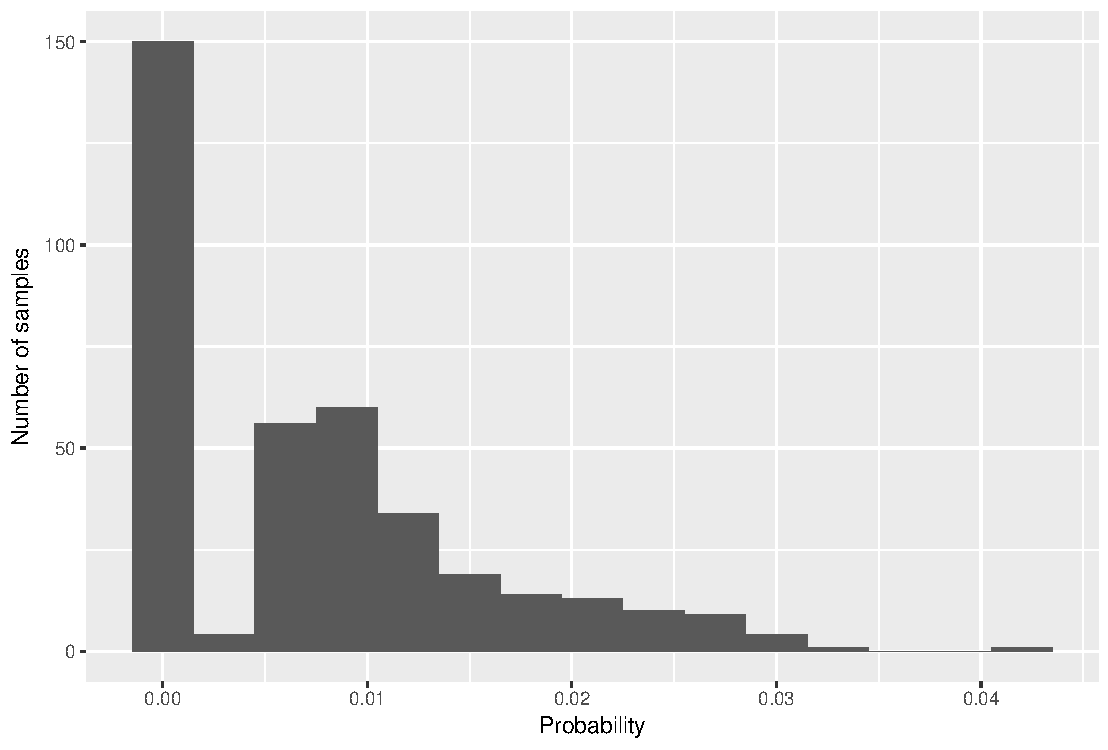
\includegraphics{Figure2-1.pdf}
\caption{\label{fig:Figure2}Frequency histogram of a STM parameter. Histogram shows
expert elicited estimates of the probability of a section of the BIFAW
transitioning from HDRG to LDRG, due to windthrow, if the ecological
thinning management option is used.}
\end{figure}

\citet{Czembor2011} used the 375 estimate sets as alternative
parameterizations to simulate BIFAW forest dynamics with the STM
software package, Vegetation Dynamics Development Tool (VDDT)
\citep{ESSA2007} running the model ten times for each scenario. Here, we
took the output from their simulations and fit MARS models for each
management action separately. Again, it was only possible to approximate
the STMs with a fast regression method as the models of each action were
fitted independently and therefore were linear with respect to the
application of the actions. Had the extra complexity of the additional
layer of dynamism been included, then using MARS to approximate the STM
models may not have been appropriate. For each of the MARS models the
response (\(n=375\times10=3750\)) was the proportion of the model
landscape in the two mature woodland states combined. The predictors
were the model parameters (including but not limited to the transition
probabilities).

All analyses were done using the statistical computing language R
version 3.3.3 \citep{R2017} with the MARS models fit (see R code
provided in online supplement for the specific model parameters used)
using the software package `earth' version 4.4.7 \citep{Milborrow2013}.

\subsection*{Calculating the Value of
Information}\label{calculating-the-value-of-information-1}
\addcontentsline{toc}{subsection}{Calculating the Value of Information}

\subsubsection*{EVPI}\label{evpi}
\addcontentsline{toc}{subsubsection}{EVPI}

To calculate EVPI we applied equations 1, 2, and 3 to the outcomes of
BIFAW management predicted by MARS models for each of the 375
alternative expert-derived parameterizations (which is equivalent to the
original simulated output of \citet{Czembor2011} averaged over the 10
model runs). These data can be transformed into a 375 by 4 matrix where
cells hold the predicted proportion of the landscape in a mature state,
with the rows representing alternative input parameter sets and columns
representing the potentially optimal solutions as in Figure
\ref{fig:Figure1}. This matrix can then be used to both calculate EVWOI
and EVWPI and by extension EVPI.

To calculate the EVWOI we first average across the rows (down the
columns) to ascertain the expected value of each potentially optimal
solution. Then choose the solution with the maximum value and this will
be the EVWOI. Calculating EVWPI requires the opposite approach. First we
work with each row individually and choose the column that maximizes the
value as if we knew with certainty that the particular parameter set,
associated with a given row, was correct. After we have maximized the
value of each of the 375 alternative scenarios, only then do we take the
average of these, which will be the EVWPI. Again the EVPI is simply the
difference between these values.

\subsubsection*{EVPXI}\label{evpxi}
\addcontentsline{toc}{subsubsection}{EVPXI}

EVPXI requires a slightly more complicated algorithm. The EVWOI in
equation 4, which is used to calculate EVPXI can be calculated as above.
However, calculating the EVWPXI for the \(i^\mathrm{th}\) parameter(s)
requires the double looping algorithm which we outline in the
pseudo-code in Box 1.

\begin{center}\rule{0.5\linewidth}{\linethickness}\end{center}

\paragraph{\texorpdfstring{Box 1: Calculating
EVWPXI\(_i\)}{Box 1: Calculating EVWPXI\_i}}\label{box-1-calculating-evwpxi_i}

To calculate EVPXI for any given parameter or parameters of interest,
which we will denote as the \(i^\mathrm{th}\) parameter(s), we apply the
following algorithm to the 375 alternative parameterizations of the 169
parameters.

\textbf{For each alternative parameterization,} \(p\), from 1 to 375.

\(\quad\) Step 1. Set parameter(s) \(i\) to parameter estimate(s)
\(p_i\).

\(\quad\) \textbf{For each each alternative parameterization,} \(p'\),
from 1 to 375.

\(\quad\) \(\quad\) Step 2. Set parameter(s) \(c\) to parameter
estimate(s) \(p'_c\).

\(\quad\) \(\quad\) Step 3. Predict the proportion of BIFAW in a mature
state with the parameters set in steps 1 and 2.

\(\quad\) \(\quad\) Step 4. Record the values of each potentially
optimal management strategy: \(Value\).

\(\quad\) \(\quad\) Repeat steps 2 to 4 above for each alternative
parameterization \(p'\).

\(\quad\) \textbf{end loop}

\(\quad\) Step 5. Average the results of step 4 across each alternative
parameterization \(p'\): \(Mean_{s_c}(Value)\).

\(\quad\) Step 6. Record the maximum average value from step 5:
\(Max_a[Mean_{s_c}(Value)]\).

\(\quad\) Repeat all steps above for each alternative parameterization
\(p\).

\textbf{end loop}

Average the result of step 6 across each alternative parameterization
\(p\): \(Mean_{s_i}\{Max_a[Mean_{s_c}(Value)]\}\).

\begin{center}\rule{0.5\linewidth}{\linethickness}\end{center}

Using the algorithm above we calculated the EVPXI for all 169
parameters. Using the same algorithm we then calculated the EVPXI for
pairs of parameters simultaneously, such that the \(i^\mathrm{th}\)
parameter was now two parameters instead of one. First we took the top
two most valuable transition probabilities that transition away from
each of the four states and calculated their joint EVPXI. Then we did
the same for the top pair of parameters for each management action. With
these results we can see which state or management action it would be
most beneficial to focus learning on.

Finally we recalculated the EVPI and EVPXI for all transition
probabilities, this time varying the constraint on the amount of ET
management allowable. This has the effect of changing the size of the
feasible management region and changing the position of the two
left-most vertices in \ref{fig:Figure1}. We recalculated the EVI for a
maximum allowable amount of thinning from 10 to 100\% in increments of
10\%.

\section*{Results}\label{results}
\addcontentsline{toc}{section}{Results}

\subsection*{MARS approximation of the state and transition
model}\label{mars-approximation-of-the-state-and-transition-model}
\addcontentsline{toc}{subsection}{MARS approximation of the state and
transition model}

The MARS models had good fit to the STM output data. The average
cross-validated (ten-fold) R\(^2\) was at least 93\% for each of the
three MARS models.

\subsection*{EVWOI: Optimal management in the face of
uncertainty}\label{evwoi-optimal-management-in-the-face-of-uncertainty}
\addcontentsline{toc}{subsection}{EVWOI: Optimal management in the face
of uncertainty}

With the original information elicited from the five experts, the
optimal decision would be to put 100\% of the BIFAW under the NM option
regardless of the constraint applied to the ET option. Given the optimal
decision is made with the original information, managers would expect,
on average, to see approximately 35\% of the BIFAW in a mature state
after 150 years. This represents a land area of 88,462 ha, a 40,962 ha
increase over the initial amount (47,500 ha, 19\%) estimated by the five
experts.

\subsection*{EVPI}\label{evpi-1}
\addcontentsline{toc}{subsection}{EVPI}

If the managers of the BIFAW had perfect knowledge and could at most,
thin 20\% of landscape, they would expect on average to see 42\% mature
woodland after 150 years (which is an EVWPI of 104,276 ha). This means
that the EVPI is 6\% or 15,814 ha (Figure \ref{fig:Figure3}). For
managers, this area of mature woodland represents the upper limit on
what resources they should be willing to spend on improving their models
of BIFAW dynamics. If the resources necessary were worth more than this
amount of mature woodland to them then it would be irrational to seek to
reduce the uncertainty.








\begin{figure}[htbp]
\centering
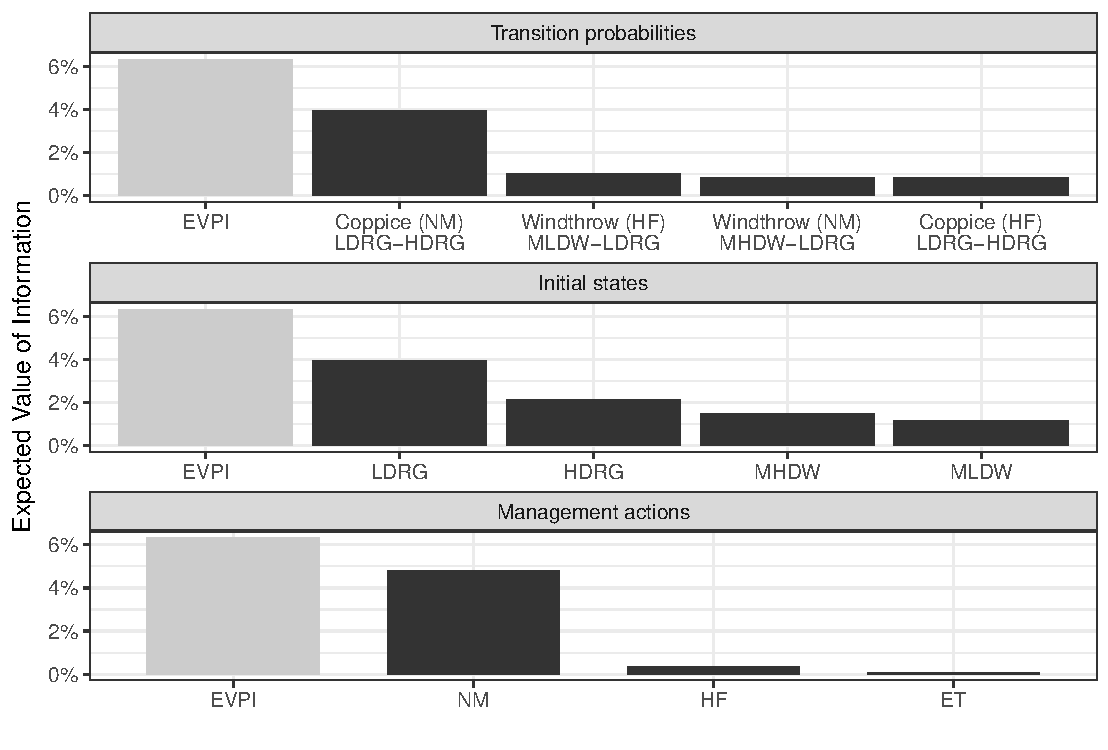
\includegraphics{Figure3-1.pdf}
\caption{\label{fig:Figure3}The expected value of partial perfect information
(EVPXI) for the top four transition probabilities on their own (top
panel), the top two transition probabilities out of each state (middle
panel) and the top two transition probabilities for each management
option (bottom panel) compared with the expected value of perfect
information (EVPI).}
\end{figure}

In calculating EVPI the 100\% NM solution was optimal 45\% of the time,
while the 100\% HF solution was only optimal 23\% of the time. Of the
solutions including 20\% ET, the solution including 80\% NM and the
solution including 80\% HF, were optimal 24\% and 8\% respectively.

\subsection*{EVPXI}\label{evpxi-1}
\addcontentsline{toc}{subsection}{EVPXI}

Of the 169 transition probabilities, most but not all, had zero or
negligible EVPXI (i.e., EVWXI\(_i\) \(\approx\) EVWOI). Figure
\ref{fig:Figure3} (top panel) shows the top four most valuable
parameters, while remaining parameters had EVPI \(<\)\%1. Notably, one
parameter (the probability of woodland transitioning from a low-density
to a high density regrowth state, due to coppicing of tree stems, when
the BIFAW is left unmanaged) was 4\%. To managers, this means if they
could completely resolve the uncertainty in this parameter alone, they
would expect to manage the BIFAW so much more optimally that on average,
they would see 9,857 ha more mature woodland in 150 years than if they
managed the forest under their initial level of uncertainty.

\subsection*{EVI when constraint on management
changes}\label{evi-when-constraint-on-management-changes}
\addcontentsline{toc}{subsection}{EVI when constraint on management
changes}

Changing the allowable amount of thinning of the BIFAW from 10 to 100\%,
that is, altering the constraint on the ET management option, changes
the EVPI and the EVPXI for some parameters (Figure \ref{fig:Figure4}).
The EVPI and the EVPXI of the most valuable transition probability
parameter (according to the analyses in the preceding section)
associated with ET increased linearly as the constraint on ET was
relaxed. The EVPI increased from 6 to 9\% while under a regime of
ecological thinning the increase in EVPXI of the probability of
transitioning from MLDW to HDRG due to fuel reduction burning was more
modest, going from 0 to 0.1\%. The EVPXI of the parameters associated
with other management options, in contrast, are invariant with respect
to the constraint on the amount of ET.






\begin{figure}[htbp]
\centering
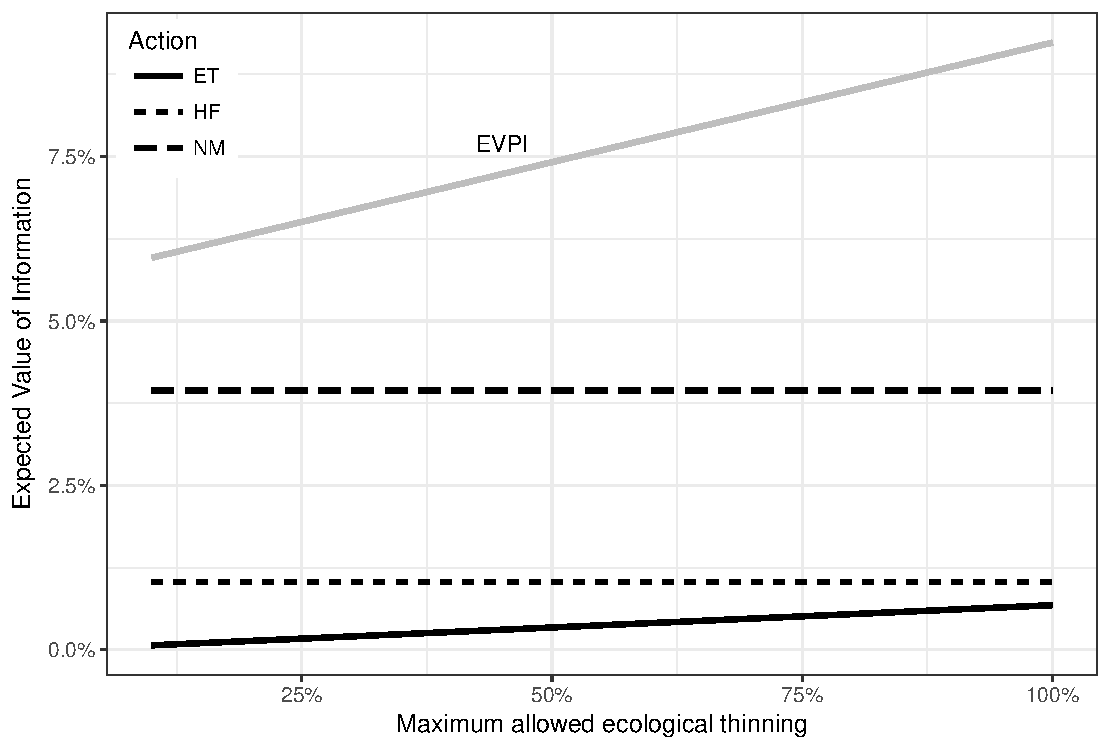
\includegraphics{Figure4-1.pdf}
\caption{\label{fig:Figure4}Response of the EVI to changing the constraint on the
allowable proportion of the BIFAW to undergo ecological thinning (ET).
The top grey line is EVPI. The three black lines are the EVPXI for the
most valuable parameter associated with each action.}
\end{figure}

\section*{Discussion}\label{discussion}
\addcontentsline{toc}{section}{Discussion}

The most important implication of these analyses for managers, is that
the most cost-effective strategies did not include either the most
desired states (mature low-density or high-density woodlands), nor what
would be thought of as the least understood management strategy
(thinning). As such, managers cannot just rely on intuition to tell them
where the most value of information is. Critical uncertainties may not
be the most uncertain, or even the uncertainties to which outcomes are
most sensitive. Critical uncertainties are the those that, when are they
reduced, can change which action is taken.

We have identified those aspects of the BIFAW system model that have the
greatest value for learning. If monitoring was targeted at the most
valuable parameter according to the EVPXI, rather than a random
parameter or even the most uncertain parameter, then the expected
performance of a subsequent decision would be greater by up to 9,857
hectares of mature woodland, given the number of management options and
constraint we used here, which is an average of 66 hectares per year.

We have also shown that if learning is targeted at subsets of the
system, so as to update multiple parameters simultaneously, then some
system states and management options would be better foci than others.
This is because the uncertainty of some parameter sets is more critical
to management decisions than others. Managers should focus learning on
the HF rather than ET or NM related parameters, because learning about
the latter options would not affect the decision outcome to as great a
degree on average. Also, if managers chose only to monitor one system
state, then learning about transitions from the LDRG state would see
greater expected benefit than the other three states. Here we have only
calculated the EVPXI for two parameters at a time, but it is possible to
include more than two parameters \citep[see
e.g.,][]{Bates2014, Bates2015}

However, the value of information depends on the number and range of
management options. In other words, the options available to manager can
drive the value of information. The greater the number and range of
management options, the greater the value of information, because the
more options you have the more potential there is for learning which
option is the best. Taken to an extreme, if you have only one option
(i.e., no decision to make) then learning would be pointless and the
value of information would be zero. In the present case, when more
thinning was permitted, EVPI and the EVPXI of the parameter predicting a
transition after thinning increased linearly, whereas the EVPXI of
parameters not associated with thinning did not change at all (Fig 3).

We caution that, to some degree, the results we obtained for our
analyses may in part be driven by limitations in the STM models, fit
previous to the current work. Lacking the non-linear dynamics of action
level interactions, and fitting separate models for each management
action, may have led to different optimal decisions and therefore
different expected values of information than if more complex and
potentially more realistic approach had been taken initially.
Nevertheless, a key advance we have made in this work is to formulate a
process for calculating VOI for complex models with continuous
expressions of uncertainty. For such models the state space is too large
to make analytical integration feasible for the VOI analyses and
numerical methods must be used instead.

However, such an approach can be computationally expensive with models
such as STMs, as it is prohibitively resource-consuming to refit a
complex model repeatedly. To overcome this, we represented the STM with
an efficient regression method (MARS) and use the output from this in
our calculations of the EVI. The method we present can be used as a
template for VOI analyses of complex models with continuous expressions
of uncertainty. Again, had a more complex STM simulation been applied
initially, the MARS approximation step we used may not have been as
successful.

The analyses we performed required us to make assumptions regarding the
monitoring to update the parameters in the model. For monitoring to take
place in the manner described, vegetation states must be able to easily
be determined in the field. In addition they must be identifiable to a
degree of accuracy that they can be distinguished from one another, so
that a transition between states is evident and recordable after
revisits occurring in a short space of time. States must not only
themselves be identifiable, but the surveyor must also be able to tell
that a unit of vegetation has been in a state for the required period of
time, for a specific transition to occur, and that any transition that
does occur has occurred due to a specific causal agent. For some
transition probabilities this set of assumptions seems plausible. For
instance, the transition from low to high-density regrowth due to
coppicing may be simple to identify and record, whereas recognizing that
a unit of vegetation remained as low-density regrowth because of
combination of drought and mistletoe may be far more difficult. This
problem arises because state-transition models are only supposed to
represent vegetation dynamics on average and do not necessarily reflect
directly observable phenomenon.

\section*{Conclusions}\label{conclusions}
\addcontentsline{toc}{section}{Conclusions}

In summary, value of information analyses could be performed to inform
monitoring and even decide whether it should take place at all. We have
shown that a value of information analysis can be used to identify which
parts of a complex model system are most valuable to address. Given the
assumptions we have outlined above and noting that our conclusions are
specific to the case we present here, managers could focus scarce
monitoring resources first on the harvest management option and the
low-density regrowth states. Here we have demonstrated how to overcome
the challenges of implementing a VOI analysis for a complex, continuous
model.

\section*{Acknowledgments}\label{acknowledgments}
\addcontentsline{toc}{section}{Acknowledgments}

We acknowledge Christina Czembor for conducting the initial research
upon which these analyses are based. We also thank Patrick Piggot and
Parks Victoria for their assistance. This work was supported by the
Australian Research Council through the Centre of Excellence in
Environmental Decisions and Linkage Project LP110100321; and the
Victorian Department of Sustainability and Environment. We thank four
anonymous reviewers for there helpful comments on earlier versions of
this work. Any use of trade, product, or firm names is for descriptive
purposes only and does not imply endorsement by the U.S. Government.

\section*{Supporting Information}\label{supporting-information}
\addcontentsline{toc}{section}{Supporting Information}

Additional supporting information, data and computer code may be found
online at \newline\texttt{ https://github.com/wkmor1/voiWoodland}

\bibliography{voiWoodland.bib}


\end{document}
